\section*{\large{DESARROLLO}}
\vspace{-0.25cm}
\justifying

\subsubsection*{\it{Sistema de control PID}}
\vspace{-0.25cm}
Para obtener una tensión de salida constante, sin importar variaciones en la tensión de entrada del
convertidor, o en la impedancia de la carga, se implementa un controlador PID.

\begin{figure}[H]
    \centering
    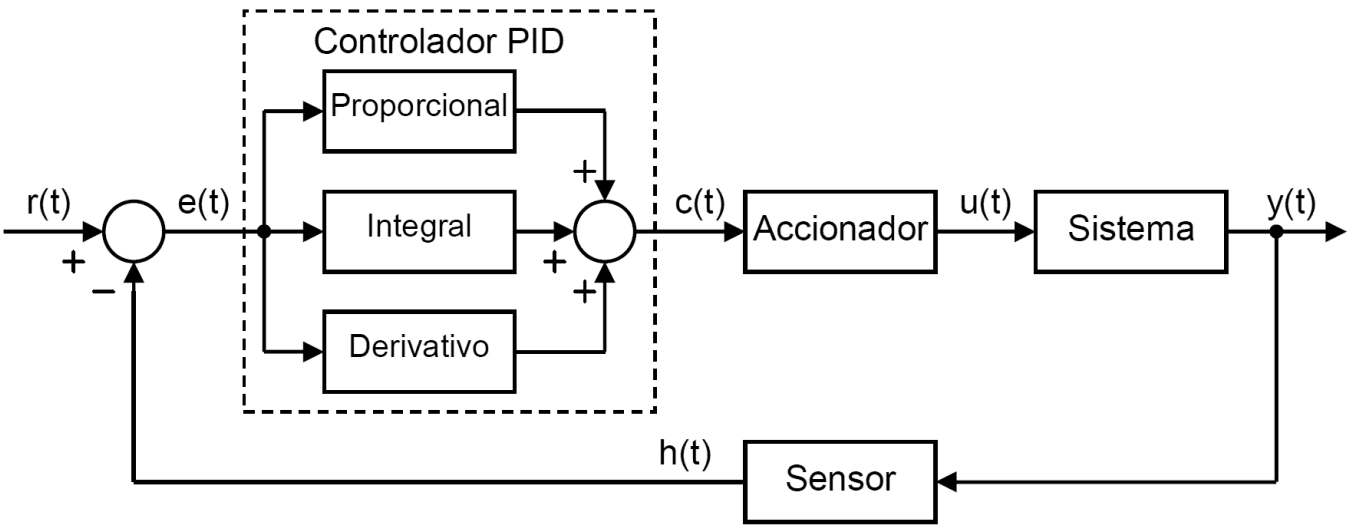
\includegraphics[height=4.5cm]{pid_diagrama.png}
    \vspace{-0.25cm}
    \caption{Diagrama de un sistema de control PID. \parencite{PICUINO}}
    \label{fig:pid_diagrama}
\end{figure}
\vspace{-0.5cm}

Donde:
\begin{itemize}[noitemsep]
    \item $r(t)$ es la señal de referencia, que indica el valor deseado a la salida del sistema.
    \item $h(t)$ es la señal de retroalimentación, que es la medición de un sensor de la salida del sistema.
    \item $e(t)$ es la señal de error, que es la diferencia entre la señal de referencia y la señal de
          retroalimentación del sistema.
    \item $c(t)$ es la señal de control, que es la salida del controlador PID.
    \item $u(t)$ es la señal de entrada al sistema.
    \item $y(t)$ es la salida del sistema.
\end{itemize}

El controlador PID consiste de tres acciones de control diferentes, que se suman para poder
obtener la señal de control. Estas acciones son:

\textbf{Acción de control proporcional (P):} es simplemente la multiplicación de la señal de error por
una constante $K_p$. Esto significa que su acción es proporcional al error. Su función de transferencia es:

\vspace{-0.5cm}
\begin{equation}
    \dfrac{U(s)}{E(s)} = K_p
\end{equation}
\vspace{-0.5cm}

\textbf{Acción de control integral (I):} es la suma acumulada de la señal de error en el tiempo, multiplicada
por una constante $K_i$. Su función de transferencia es:

\vspace{-0.5cm}
\begin{equation}
    \dfrac{U(s)}{E(s)} = \dfrac{K_i}{s}
\end{equation}
\vspace{-0.5cm}

\textbf{Acción de control derivativa (D):} es la derivada de la señal de error en el tiempo, multiplicada por
una constante $K_d$. Su función de transferencia es:

\vspace{-0.5cm}
\begin{equation}
    \dfrac{U(s)}{E(s)} = K_d \cdot s
\end{equation}
\vspace{-0.5cm}

Para reducir el ruido de alta frecuencia en la señal de control, así como para evitar inestabilidades
en el sistema, se utiliza un filtro pasa-bajos en la acción derivativa. La función de transferencia es:

\vspace{-0.5cm}
\begin{equation}
    \dfrac{U(s)}{E(s)} = K_d \cdot \dfrac{N}{1+\dfrac{N}{s}}
\end{equation}
\vspace{-0.5cm}

Sumando las tres acciones de control, obtenemos la función de transferencia en forma paralela del controlador PID:

\vspace{-0.5cm}
\begin{equation}
    \dfrac{U(s)}{E(s)} = K_p + \dfrac{K_i}{s} + K_d \cdot \dfrac{N}{1+\dfrac{N}{s}}
\end{equation}
\vspace{-0.5cm}

Como en nuestro sistema de control se utiliza un microcontrolador, se debe discretizar la función de transferencia
del controlador PID para implementarla correctamente. Utilizando la transformación de Euler, se obtiene la siguiente
función de transferencia discreta:

\vspace{-0.5cm}
\begin{equation}
    \dfrac{U(s)}{E(s)} = K_p + K_i \cdot \dfrac{T_s}{z-1} + K_d \cdot \dfrac{N}{1+N \cdot \dfrac{T_s}{z-1}}
\end{equation}
\vspace{-0.5cm}

Aplicando denominador común y agrupando términos, se obtiene:

\vspace{-0.5cm}
\begin{equation}
    \dfrac{U(z)}{E(z)} =
    \frac
    {
        \splitfrac{
            (K_p + K_d N)\ z^2 + (-2 K_p - 2 K_d N + K_i T_s + K_p N T_s)\ z
        }{
            + (K_p + K_d N - K_i T_s - K_p N T_s + K_i N {T_s}^2)
        }
    }
    {
            z^2 + (-2 + N T_s) z + (1 - N T_s)
    }
    \end{equation}
\vspace{-0.5cm}

Finalmente, se puede obtener la ecuación en diferencias del controlador PID:

\vspace{-0.5cm}
\begin{multline}
        u[n] = (K_p + K_d N)\ e[n] + (-2 K_p - 2 K_d N + K_i T_s + K_p N T_s)\ e[n-1]\  + \\
    (K_p + K_d N - K_i T_s - K_p N T_s + K_i N {T_s}^2)\ e[n-2] - (2 - N T_s)\ u[n-1] - (1 - N T_s)\ u[n-2]
\end{multline}
\vspace{-0.5cm}

\subsubsection*{\it{Modelado del sistema}}
\vspace{-0.25cm}

El sistema convertidor Buck es un sistema conmutado. Consta de dos estados de conmutación: 
en primer lugar, cuando el interruptor está conectado al nodo 1, estado de carga; en segundo lugar, cuando
el interruptor está conectado al nodo 2, estado de descarga.
El sistema conmutado se puede modelar como un sistema promediado.

\begin{figure}[H]
    \centering
    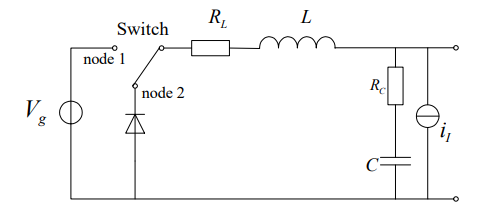
\includegraphics[height=4.5cm]{modelado_circuito.png}
    \vspace{-0.25cm}
    \caption{Circuito general del sistema.}
    \label{fig:modelado_circuito}
\end{figure}

Primero, la fuente se incluye en el circuito cuando el interruptor esta conectado al nodo 1.

\begin{figure}[H]
    \centering
    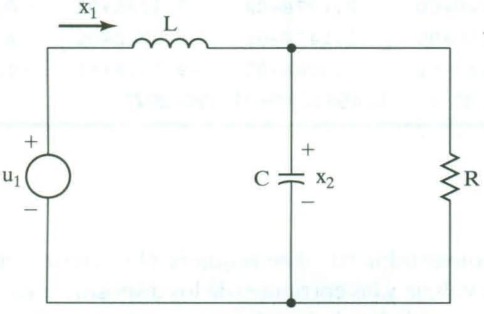
\includegraphics[height=4.5cm]{modelo_con_vg.png}
    \vspace{-0.25cm}
    \caption{Circuito con fuente de voltaje.}
    \label{fig:modelado_con_vg}
\end{figure}

Aplicando ley de Kirchoff obtenemos:

\vspace{-0.5cm}
\begin{equation}
    u_1 = Lx'_1 + x_2
\end{equation}

\vspace{-0.5cm}
\begin{equation}
    Cx'_2 = x_1 - \dfrac{1}{R} x_2 
\end{equation}

Donde $x_1$ es la corriente que circula por el inductor, $x_2$ es la tensión en el capacitor y $u_1$ la tensión de entrada.
Reordenando nos queda:

\vspace{-0.5cm}
\begin{equation}
    x'_1 = -\dfrac{1}{L} x_2 + \dfrac{1}{L} u_1
\end{equation}

\vspace{-0.5cm}
\begin{equation}
    x'_2 = \dfrac{1}{C}x_1 - \dfrac{1}{RC} x_2 
\end{equation}

De aqui podemos obtener las matrices $A_1$ y $B_1$:

\begin{equation}
    A_1 = \begin{bmatrix}
        0 & -\dfrac{1}{L}\\
        \dfrac{1}{C} & -\dfrac{1}{RC}
    \end{bmatrix}
\end{equation}

\begin{equation}
    B_1 = \begin{bmatrix}
        \dfrac{1}{L}\\
        0
    \end{bmatrix}
\end{equation}

Cuando el interruptor esta conectado al nodo dos, las fuente de tensión 
no se incluye en el circuito.

\begin{figure}[H]
    \centering
    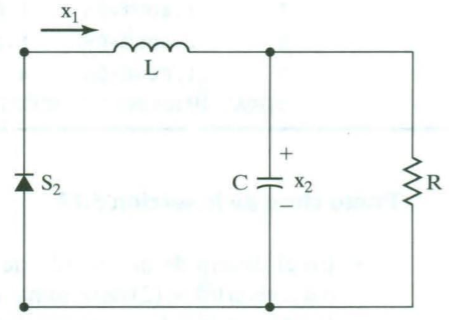
\includegraphics[height=4.5cm]{modelo_sin_vg.png}
    \vspace{-0.25cm}
    \caption{Circuito sin fuente de voltaje.}
    \label{fig:modelado_sin_vg}
\end{figure}

Nuevamente aplicando ley de Kirchoff, y reordenando las ecuaciones:

\vspace{-0.5cm}
\begin{equation}
    0 = Lx'_1 + x_2
\end{equation}

\vspace{-0.5cm}
\begin{equation}
    Cx'_2 = x_1 - \dfrac{1}{R} x_2 
\end{equation}

\vspace{-0.5cm}
\begin{equation}
    x'_1 = -\dfrac{1}{L} x_2
\end{equation}

\vspace{-0.5cm}
\begin{equation}
    x'_2 = \dfrac{1}{C} x_1 - \dfrac{1}{RC} x_2 
\end{equation}

De aqui podemos obtener las matrices $A_2$ y $B_2$:

\begin{equation}
    A_2 = \begin{bmatrix}
        0 & -\dfrac{1}{L}\\
        \dfrac{1}{C} & -\dfrac{1}{RC}
    \end{bmatrix}
\end{equation}

\begin{equation}
    B_2 = \begin{bmatrix}
        0\\
        0
    \end{bmatrix}
\end{equation}

Para los dos casos, las salida es igual a la tension en el capacitor, $x_2$:

\vspace{-0.5cm}
\begin{equation}
    y = \begin{bmatrix}
        0 & 1
    \end{bmatrix}
    \cdot
    \begin{bmatrix}
        x_1 \\
        x_2
    \end{bmatrix}
\end{equation}

\textbf{Obtención del sistema promediado:}

La solución total se puede obtener promediando en espacio de estados, esto es, sumando los términos 
para cada análisis del modo lineal conmutado. Como solo cambia la matriz B, se hace sobre esa unica matriz.
Suponiendo el ciclo de trabajo d, tenemos:

\vspace{-0.5cm}
\begin{equation}
    B_{Promedio} = d \cdot B_1 + (1 - d) \cdot B_2
\end{equation}

Sustituyendo obtenemos la matriz A, B y C del sistema:

\begin{equation}
    A = \begin{bmatrix}
        0 & -\dfrac{1}{L}\\
        \dfrac{1}{C} & -\dfrac{1}{RC}
    \end{bmatrix}
\end{equation}

\begin{equation}
    B = \begin{bmatrix}
        \dfrac{d}{L}\\
        0
    \end{bmatrix}
\end{equation}

\begin{equation}
    C = \begin{bmatrix}
        0 & 1
    \end{bmatrix}
\end{equation}

Lo que resulta en el siguiente sistema de estado:

\vspace{-0.5cm}
\begin{equation}
    \begin{cases}
        \begin{bmatrix}
            \dot{x_1}\\
            \dot{x_2}
        \end{bmatrix}
        =
        \begin{bmatrix}
            0  &   -\dfrac{1}{L}\\
            \dfrac{1}{C} & -\dfrac{1}{RC}
        \end{bmatrix}
        \cdot
        \begin{bmatrix}
            x_1 \\
            x_2
        \end{bmatrix}
        +
        \begin{bmatrix}
            \dfrac{d}{L} \\
            0
        \end{bmatrix}
        \cdot
        u_1 
        \\
        \\
        y =
        \begin{bmatrix}
            0 & 1
        \end{bmatrix}
        \cdot
        \begin{bmatrix}
            x_1 \\
            x_2
        \end{bmatrix}

    \end{cases}
\end{equation}

Aunque el sistema original es lineal para toda condición dada de conmutación, el sistema que resulta 
en general es no lineal debido a que el ciclo de trabajo d es en general una función de $x_1$, $x_2$ y $u_1$. \parencite{RASHID}


\subsubsection*{\it{Circuito}}
\vspace{-0.25cm}

Para construir el circuito físico, primero se realizó el siguiente diagrama:

\begin{figure}[H]
    \centering
    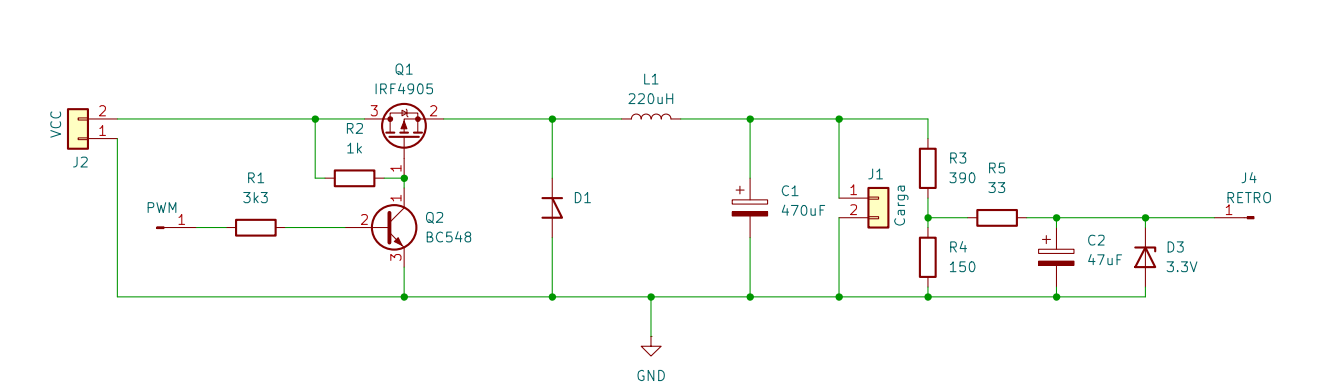
\includegraphics[height=4.5cm]{diagrama_circuito.png}
    \vspace{-0.25cm}
    \caption{Diagrama de circuito.}
    \label{fig:diagrama_circuito}
\end{figure}

Los componentes fuero seleccionados según disponibilidad y costos, teniendo en cuenta que cumplan los requerimientos del circuito.
El divisor resistivo que conecta la retroalimentación al microcontrolador esta diseñado para que entregue una 
tensión de 0 V a 3,3 V. Para ello se realizo una tabla con valores de entrada y salida:

\begin{table}[H]
    \centering
    \begin{tabular}{|c|c|}
    \hline
    Voltaje de retroalimentación (V) & Tensión en la carga (V) \\ \hline
    0                                & 0                       \\
    0.27                             & 1                       \\
    0.55                             & 2                       \\
    0.83                             & 3.05                    \\
    1.07                             & 3.9                     \\
    1.38                             & 5.01                    \\
    1.66                             & 6.03                    \\
    1.95                             & 7.09                    \\
    2.19                             & 8.02                    \\
    2.44                             & 9.06                    \\
    2.65                             & 9.96                    \\
    2.87                             & 11                      \\
    3.04                             & 12                      \\ \hline
    \end{tabular}
    \label{tab:calibración_fb}
    \vspace{-0.25cm}
    \caption{Calibración de voltaje de retroalimentación}
\end{table}

\subsubsection*{\it{Identificación del sistema}}
\vspace{-0.25cm}
Si bien el modelo del sistema se puede obtener a partir de las ecuaciones de Kirchhoff, se procede
a obtener un modelo empírico. Para ello, se aplica una señal de entrada al sistema físico y se
mide la respuesta del mismo.

En esta ocasión, se optó por utilizar una señal de entrada PRBS
(Pseudo Random Binary Sequence, en español Secuencia Binaria Pseudo Aleatoria). La misma intenta
cubrir todo el rango de frecuencias posibles, y es útil para identificar sistemas lineales y no lineales.
Utilizando MATLAB, se genera una señal PRBS con un tiempo de muestreo de 200 microsegundos, frecuencia máxima
800 Hz, y una duración de 10 períodos. Esta señal es una secuencia de 186 valores en 0,0372 segundos repetida diez veces.
Es decir, 1860 valores en un rango de 0 a 0,372 segundos.

Se programa el microcontrolador para reproducir la señal PRBS en el convertidor Buck, medir la salida
del sistema y luego enviar los datos mediante comunicación serial. A través de un programa en Python, se guardan
los valores en un archivo csv para luego introducir en el System Identification Toolbox de MATLAB:


\begin{figure}[H]
    \centering

    \begin{subfigure}[b]{\textwidth}
        \centering
        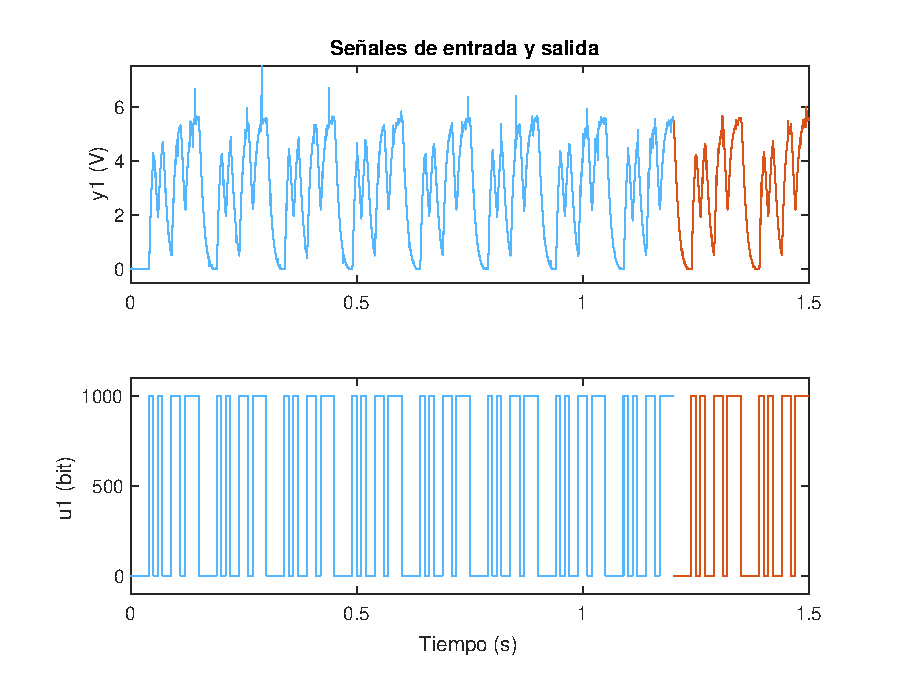
\includegraphics[height=8cm]{identificacion_io.eps}
        %\vspace{-0.25cm}
        \caption{Vista completa de la señal de identificación.}
        \label{fig:identificacion_io_gral}
    \end{subfigure}
    \begin{subfigure}[b]{\textwidth}
        \centering
        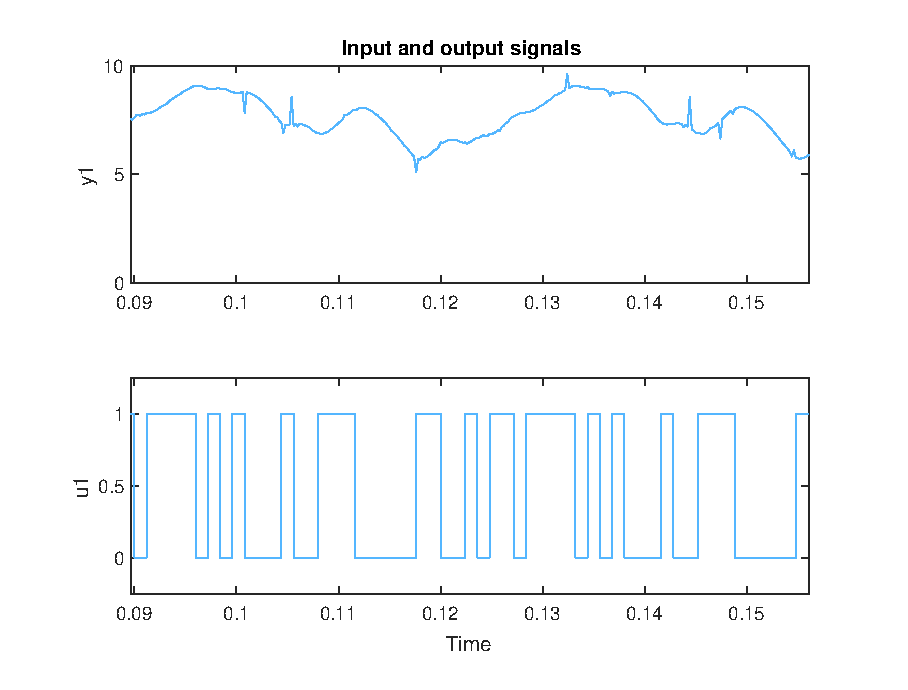
\includegraphics[height=8cm]{identificacion_zoom.eps}
        %\vspace{-0.25cm}
        \caption{Vista acercada de la señal de identificación.}
        \label{fig:identificacion_io_zoom}
    \end{subfigure}

    \vspace{-0.25cm}
    \caption{Salida (arriba) y entrada (abajo) del sistema con la señal de identificación.}
    \label{fig:identificacion_io}
\end{figure}
\vspace{-0.5cm}

Se seleccionan los primeros 1488 valores (80\% de los valores totales) como la señal de evaluación
y los restantes 372 valores (20\% de los valores totales) como la señal de validación. Finalmente,
se estima un modelo en espacios de estado de orden 3 utilizando la función \textit{N4SID} del System Identification Toolbox:

\begin{figure}[H]
    \centering

    \begin{subfigure}[b]{\textwidth}
        \centering
        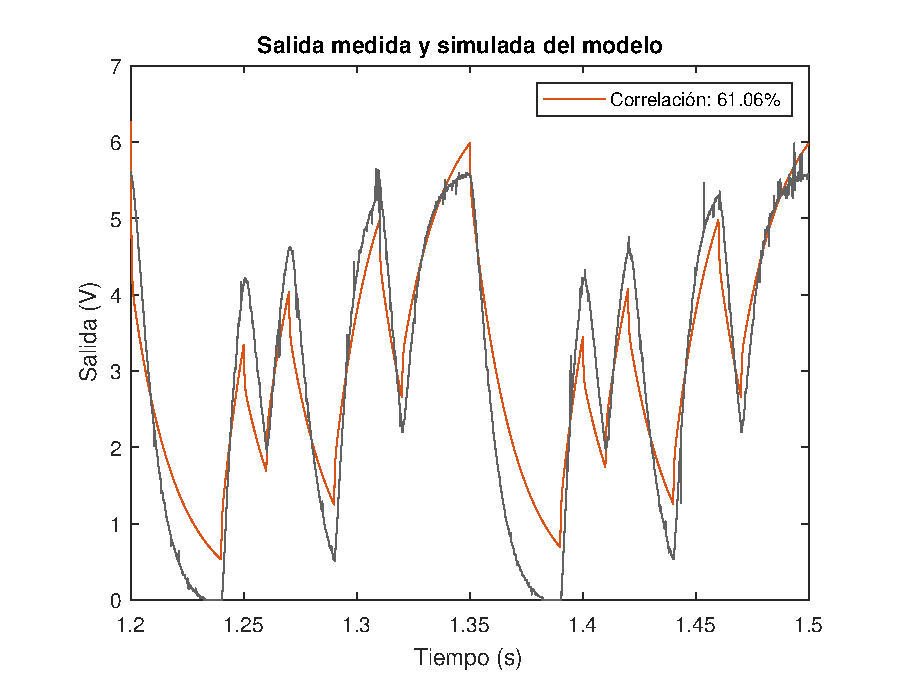
\includegraphics[width=10cm]{identificacion_comparacion.eps}
        %\vspace{-0.25cm}
        \caption{Comparación del modelo estimado con la respuesta medida.}
        \vspace{0.25cm}
        \label{fig:identificacion_comparacio n}
    \end{subfigure}
    \begin{subfigure}[b]{\textwidth}
        \centering
        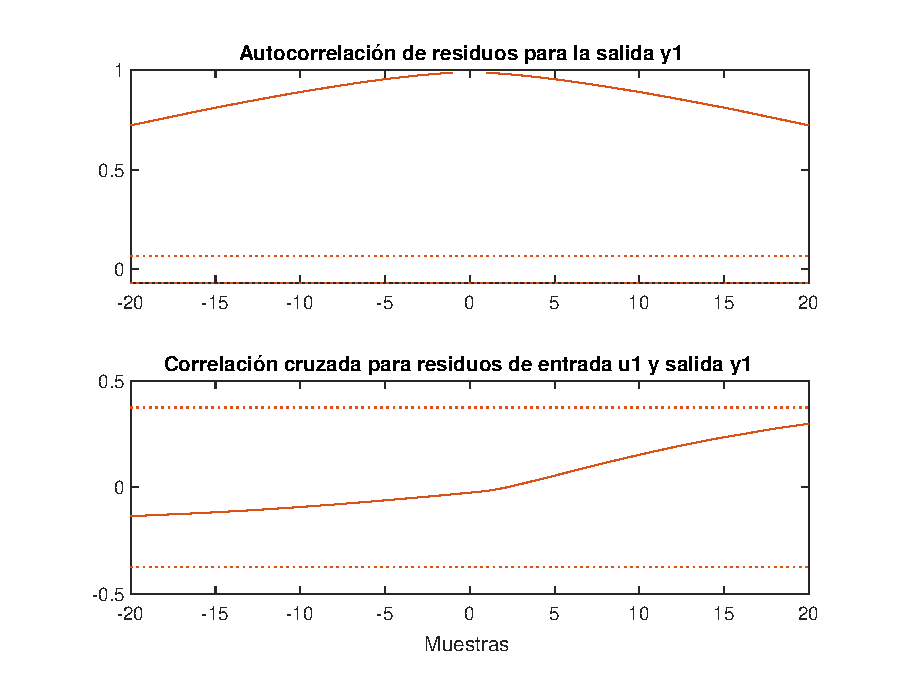
\includegraphics[width=10cm]{identificacion_residuos.eps}
        %\vspace{-0.25cm}
        \caption{Análisis residual del modelo estimado.}
        \label{fig:identificacion_residuos}
    \end{subfigure}

    \vspace{-0.25cm}
    \caption{Resultados de la estimación del modelo del sistema.}
    \label{fig:identificacion_resultados}
\end{figure}
\vspace{-0.5cm}

Como se puede observar en la Figura \ref{fig:identificacion_resultados}, el modelo estimado coincide
con la respuesta medida del sistema (señal de validación) en un 64,     89\%. Respecto a la señal de 
evaluación, coincide en un 92,61\%. Además, el análisis residual del modelo estimado
demuestra un buen resultado en la autocorrelación de residuales para la salida y para la correlación
cruzada de residuales entre la entrada y la salida.

El modelo estimado en espacios de estado es el siguiente:

\vspace{-0.5cm}
\begin{equation}
    \begin{cases}
        \begin{bmatrix}
            \dot{x_1}   \\
            \dot{x_2}   \\
            \dot{x_3}
        \end{bmatrix}
        =
        \begin{bmatrix}
            0.9933   &   -0.01093    &   -0.0006102\\
            0.1064   &   0.8617      &   -0.2955   \\
            0.005556 &   -0.02709    &   -0.6608            
        \end{bmatrix}
        \begin{bmatrix}
            x_1 \\
            x_2 \\
            x_3
        \end{bmatrix}
        +
        \begin{bmatrix}
            0.000438   \\
            -0.005044  \\
            0.02667
        \end{bmatrix}
        u 
        +
        \begin{bmatrix}
            0.002016 \\
            -0.0145   \\
            -0.008185
        \end{bmatrix}
        e
        \\
        y =
        \begin{bmatrix}
            188.4 & 2.647 & 0.7808
        \end{bmatrix}

        \begin{bmatrix}
            x_1 \\
            x_2 \\
            x_3
        \end{bmatrix}
        +
        e

    \end{cases}
\end{equation}

El mismo se puede representar en función de transferencia luego de transformarlo mediante MATLAB:

\vspace{-0.5cm}
\begin{equation}
    H(s) = \dfrac{3062\ s + 1.456 \times 10^7}{s^2 + 1.199 \times 10^4\ s + 1.722 \times 10^6}
\end{equation}
\vspace{-0.5cm}

La planta discretizada mediante retención de orden cero (zoh), con un tiempo de muestreo de 200
microsegundos es:

\vspace{-0.5cm}
\begin{equation}
    H(z) = \dfrac{0.3798\ z - 0.1602}{z^2 - 1.065\ z + 0.09091}
\end{equation}
\vspace{-0.5cm}

A continuación se grafican las respuestas al impulso y al escalón, el mapa de polos y ceros y el lugar
geométrico de las raíces.

\begin{figure}[H]
    \centering

    \begin{subfigure}[b]{0.49\textwidth}
        \centering
        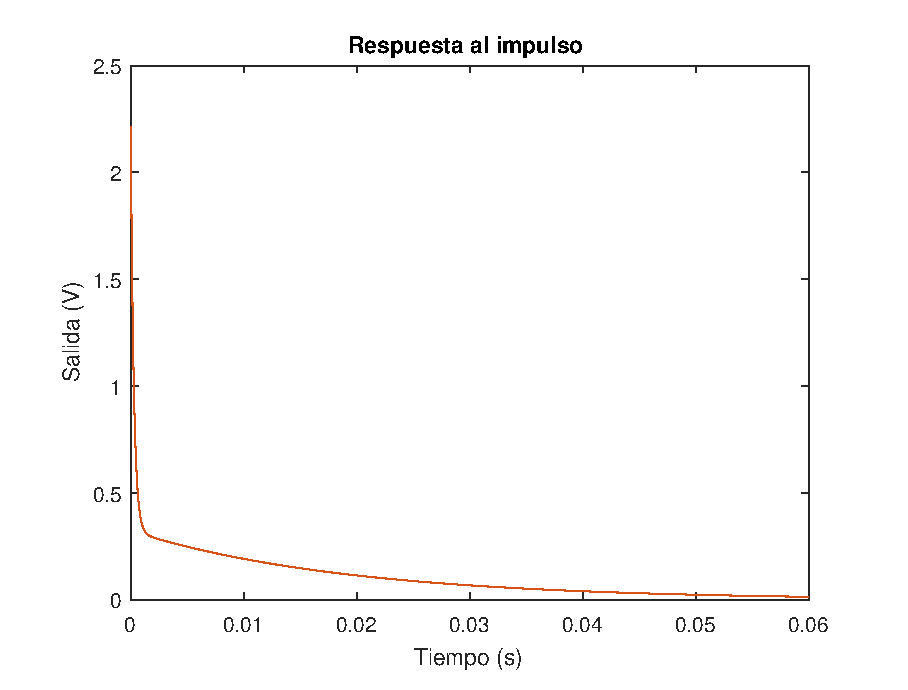
\includegraphics[width=\textwidth]{estimado_impulse.eps}
        %\vspace{-0.25cm}
        \caption{Respuesta al impulso.}
        \label{fig:estimado_impulse}
    \end{subfigure}
    \begin{subfigure}[b]{0.49\textwidth}
        \centering
        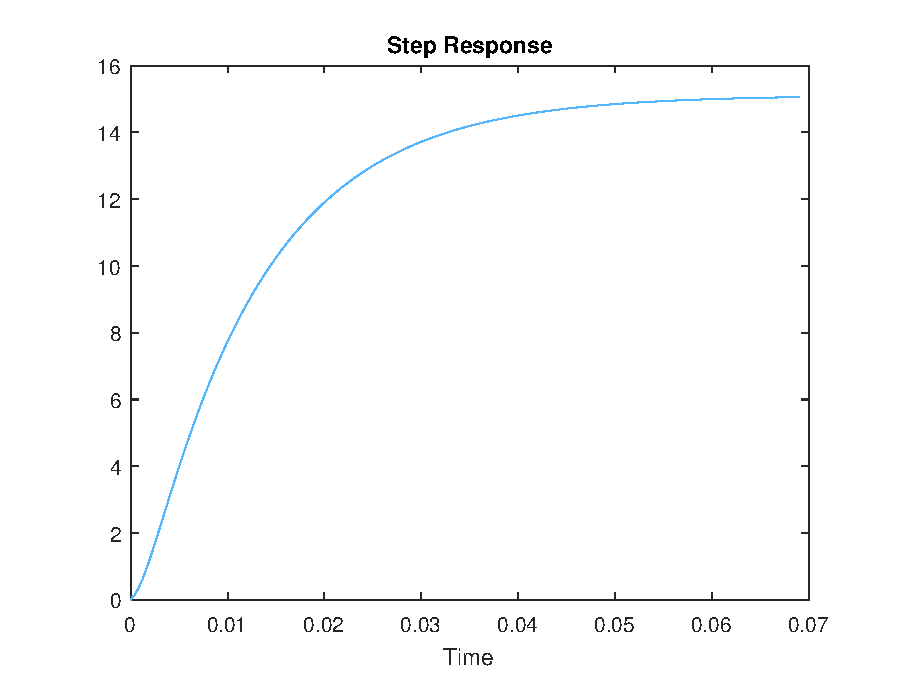
\includegraphics[width=\textwidth]{estimado_step.eps}
        %\vspace{-0.25cm}
        \caption{Respuesta al escalón.}
        \label{fig:estimado_step}
    \end{subfigure}

    \vspace{-0.25cm}
    \caption{Análisis de la respuesta temporal del sistema estimado.}
    \label{fig:estimado_respuestas}
\end{figure}
\vspace{-0.5cm}

\begin{figure}[H]
    \centering

    \begin{subfigure}[b]{0.49\textwidth}
        \centering
        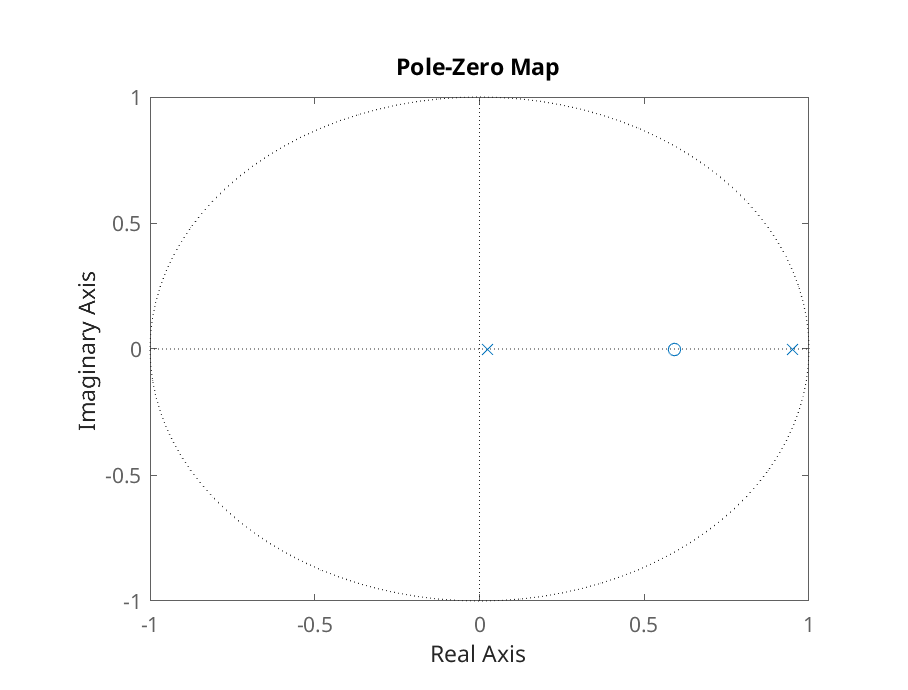
\includegraphics[width=\textwidth]{estimado_pzmap.eps}
        %\vspace{-0.25cm}
        \caption{Mapa de polos y ceros.}
        \label{fig:estimado_pzmap}
    \end{subfigure}
    \begin{subfigure}[b]{0.49\textwidth}
        \centering
        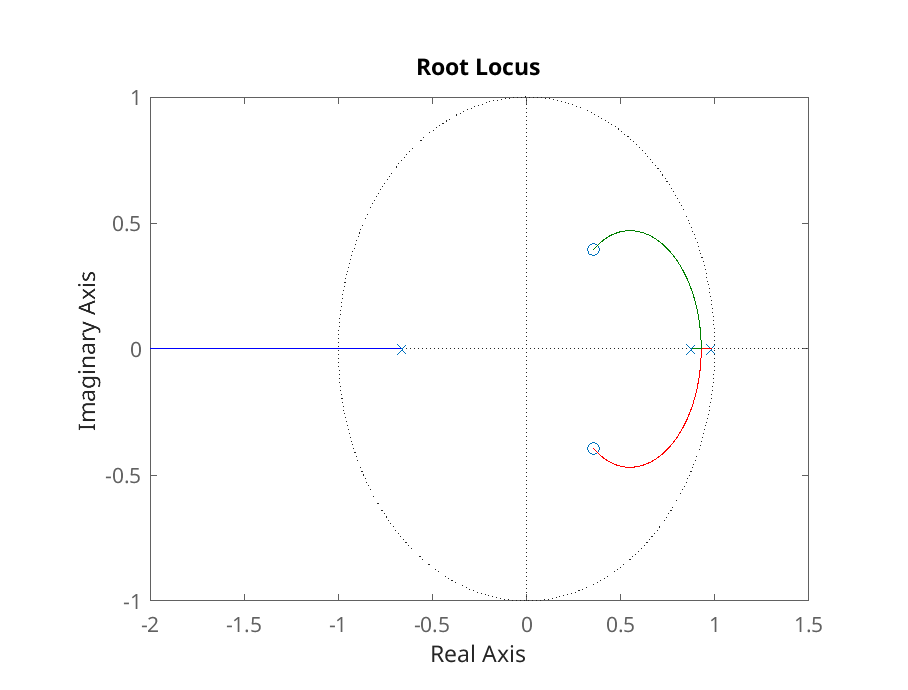
\includegraphics[width=\textwidth]{estimado_rlocus.eps}
        %\vspace{-0.25cm}
        \caption{Lugar geométrico de las raíces.}
        \label{fig:estimado_rlocus}
    \end{subfigure}

    \vspace{-0.25cm}
    \caption{Análisis de la respuesta temporal del sistema estimado.}
    \label{fig:estimado_estabilidad}
\end{figure}
\vspace{-0.5cm}

La respuesta al impulso del sistema converge a cero cuando el tiempo tiende al infinito.
En la respuesta al escalón, el sistema converge a un valor.
La ubicación de polos y el lugar geométricos de las raíces están ubicados dentro 
del circulo unitario en el plano z. Debido a estas características se determina que el sistema 
es estable.